\magnification=\magstep1
\input epsf.tex
\input psfrag
\newdimen\epsfxsize
\newdimen\epsfysize


\nopagenumbers
\centerline{\bf Worksheet 8 --- Math 126 -- Summer 2010}
\bigskip
\item{1.}
Use the Taylor Series  for the exponential function
to do the following.
      \itemitem{(a)} Find the Taylor Series based at zero for
                $f(x) = e^{x^3 - 1} = e^{x^3}/e$.
                What is the value of ${{d^{15}f}\over{dx ^{15}}}$ at $x=0$?
%% Could change everything to T. plys instead of series,  then in
%% part a above, say find 6th taylor poly, what will the x^15 term be
%% in the 15th taylor poly? Similarly for rest of questions.

       \itemitem{(b)} Find the Taylor Series based at zero for
                $g(x) = e^{(x/a)^2 - b}$.
        \itemitem{(c)} Find the Taylor Series based at zero for
                $h(x) = xe^{(x/a)^2 - b}$.
        Hint:  How is $h$ related to $g$ in part (b)?
       \itemitem{(d)} Find the Taylor Series based at $1$ for
                $f(x) = xe^x$.

\bigskip
Here is an application of Taylor polynomials:
\bigskip
\item{2.} An electric dipole consists of two electric charges of equal magnitude
and opposite signs. If the charges are $q$ and $-q$ and are located at
a distance $d$ from each other, then the electric field $E$ at the
point $P$ in the figure 

\bigskip
\psfrag{D}{$D$}
\psfrag{d}{$d$}
\psfrag{q}{$q$}
\psfrag{mq}{$-q$}
\psfrag{P}{$P$}

\centerline{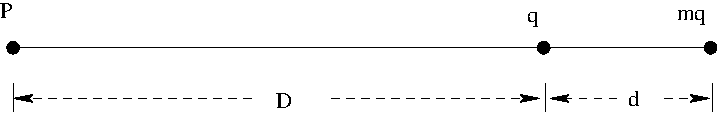
\includegraphics[width=2.25in]{dipole}}

\bigskip
is given by


$$E={{q}\over {D^2}} - {{q}\over{(D+d)^2}}={{q}\over{D^2}}
\biggl[1-{{1}\over{(1+{d\over D})^2}}\biggl].$$

\bigskip
\item{}Treating $d/D$ as a variable (set $x=d/D$) write down the Taylor
expansion (Taylor Series) for the function 
inside the square brackets.
Multiply the Taylor expansion by $q/D^2$ to obtain an expansion for
$E$. Using the expansion you obtained, show that $E$ is approximately
$2qd/(D^3)$ when $P$ is far away from the dipole.

\bigskip

\item{} Comment: The electric field decays much more rapidly
than the field generated by one of the charges because the fields
generated by each particle partially
cancel one another. The approximation tells us the rate of
decay.

\end
